% Created by tikzDevice version 0.12.3.1 on 2021-07-01 12:50:32
% !TEX encoding = UTF-8 Unicode
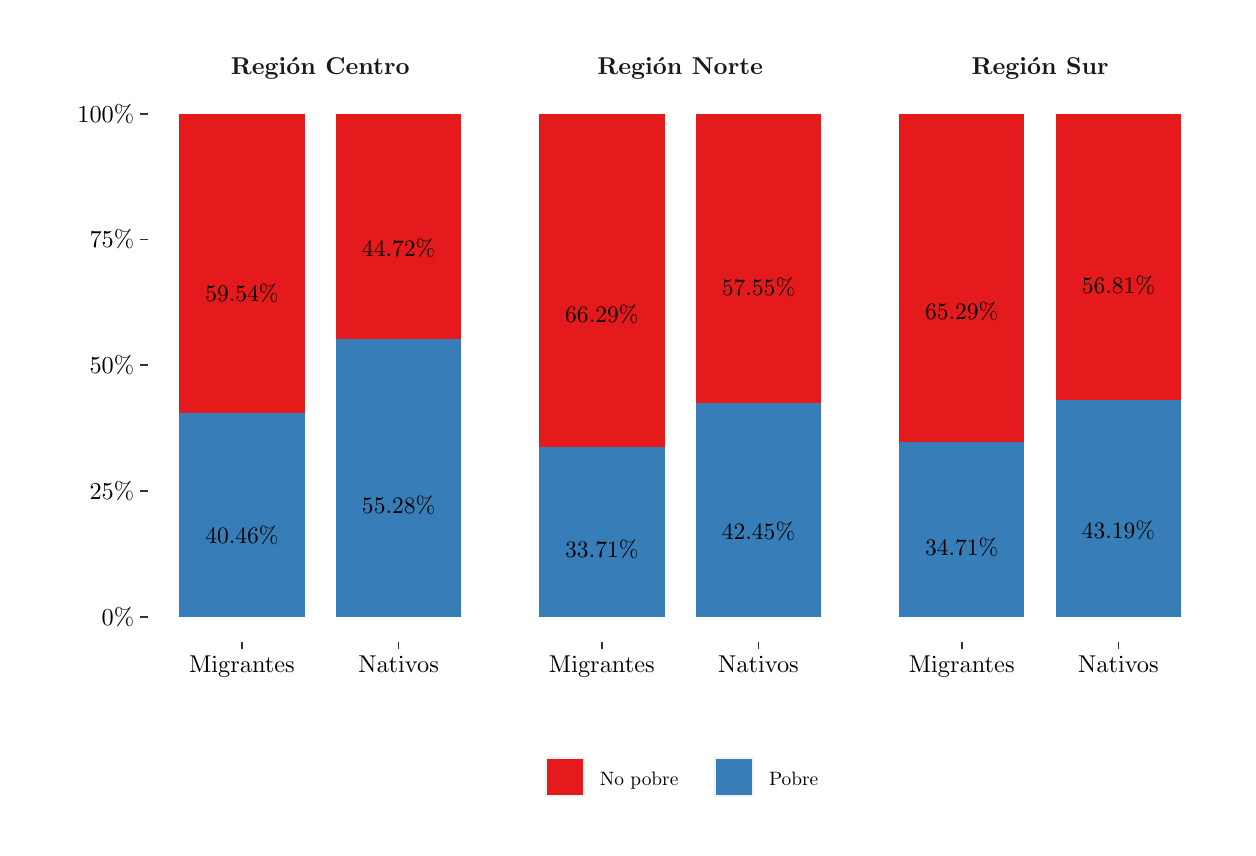
\begin{tikzpicture}[x=1pt,y=1pt]
\definecolor{fillColor}{RGB}{255,255,255}
\path[use as bounding box,fill=fillColor,fill opacity=0.00] (0,0) rectangle (433.62,289.08);
\begin{scope}
\path[clip] (  0.00,  0.00) rectangle (433.62,289.08);
\definecolor{drawColor}{RGB}{255,255,255}
\definecolor{fillColor}{RGB}{255,255,255}

\path[draw=drawColor,line width= 0.6pt,line join=round,line cap=round,fill=fillColor] (  0.00, -0.00) rectangle (433.62,289.08);
\end{scope}
\begin{scope}
\path[clip] ( 43.44, 67.14) rectangle (168.00,267.01);
\definecolor{drawColor}{RGB}{255,255,255}

\path[draw=drawColor,line width= 0.3pt,line join=round] ( 43.44, 98.94) --
	(168.00, 98.94);

\path[draw=drawColor,line width= 0.3pt,line join=round] ( 43.44,144.36) --
	(168.00,144.36);

\path[draw=drawColor,line width= 0.3pt,line join=round] ( 43.44,189.79) --
	(168.00,189.79);

\path[draw=drawColor,line width= 0.3pt,line join=round] ( 43.44,235.21) --
	(168.00,235.21);

\path[draw=drawColor,line width= 0.6pt,line join=round] ( 43.44, 76.22) --
	(168.00, 76.22);

\path[draw=drawColor,line width= 0.6pt,line join=round] ( 43.44,121.65) --
	(168.00,121.65);

\path[draw=drawColor,line width= 0.6pt,line join=round] ( 43.44,167.07) --
	(168.00,167.07);

\path[draw=drawColor,line width= 0.6pt,line join=round] ( 43.44,212.50) --
	(168.00,212.50);

\path[draw=drawColor,line width= 0.6pt,line join=round] ( 43.44,257.92) --
	(168.00,257.92);

\path[draw=drawColor,line width= 0.6pt,line join=round] ( 77.41, 67.14) --
	( 77.41,267.01);

\path[draw=drawColor,line width= 0.6pt,line join=round] (134.03, 67.14) --
	(134.03,267.01);
\definecolor{fillColor}{RGB}{228,26,28}

\path[fill=fillColor] ( 54.77,149.74) rectangle (100.06,257.92);
\definecolor{fillColor}{RGB}{55,126,184}

\path[fill=fillColor] ( 54.77, 76.22) rectangle (100.06,149.74);
\definecolor{fillColor}{RGB}{228,26,28}

\path[fill=fillColor] (111.38,176.68) rectangle (156.68,257.92);
\definecolor{fillColor}{RGB}{55,126,184}

\path[fill=fillColor] (111.38, 76.22) rectangle (156.68,176.68);
\definecolor{drawColor}{RGB}{0,0,0}

\node[text=drawColor,anchor=base,inner sep=0pt, outer sep=0pt, scale=  0.85] at ( 77.41,190.07) {59.54{\%}};

\node[text=drawColor,anchor=base,inner sep=0pt, outer sep=0pt, scale=  0.85] at ( 77.41,102.69) {40.46{\%}};

\node[text=drawColor,anchor=base,inner sep=0pt, outer sep=0pt, scale=  0.85] at (134.03,206.24) {44.72{\%}};

\node[text=drawColor,anchor=base,inner sep=0pt, outer sep=0pt, scale=  0.85] at (134.03,113.47) {55.28{\%}};
\end{scope}
\begin{scope}
\path[clip] (173.50, 67.14) rectangle (298.06,267.01);
\definecolor{drawColor}{RGB}{255,255,255}

\path[draw=drawColor,line width= 0.3pt,line join=round] (173.50, 98.94) --
	(298.06, 98.94);

\path[draw=drawColor,line width= 0.3pt,line join=round] (173.50,144.36) --
	(298.06,144.36);

\path[draw=drawColor,line width= 0.3pt,line join=round] (173.50,189.79) --
	(298.06,189.79);

\path[draw=drawColor,line width= 0.3pt,line join=round] (173.50,235.21) --
	(298.06,235.21);

\path[draw=drawColor,line width= 0.6pt,line join=round] (173.50, 76.22) --
	(298.06, 76.22);

\path[draw=drawColor,line width= 0.6pt,line join=round] (173.50,121.65) --
	(298.06,121.65);

\path[draw=drawColor,line width= 0.6pt,line join=round] (173.50,167.07) --
	(298.06,167.07);

\path[draw=drawColor,line width= 0.6pt,line join=round] (173.50,212.50) --
	(298.06,212.50);

\path[draw=drawColor,line width= 0.6pt,line join=round] (173.50,257.92) --
	(298.06,257.92);

\path[draw=drawColor,line width= 0.6pt,line join=round] (207.47, 67.14) --
	(207.47,267.01);

\path[draw=drawColor,line width= 0.6pt,line join=round] (264.09, 67.14) --
	(264.09,267.01);
\definecolor{fillColor}{RGB}{228,26,28}

\path[fill=fillColor] (184.83,137.47) rectangle (230.12,257.92);
\definecolor{fillColor}{RGB}{55,126,184}

\path[fill=fillColor] (184.83, 76.22) rectangle (230.12,137.47);
\definecolor{fillColor}{RGB}{228,26,28}

\path[fill=fillColor] (241.44,153.36) rectangle (286.74,257.92);
\definecolor{fillColor}{RGB}{55,126,184}

\path[fill=fillColor] (241.44, 76.22) rectangle (286.74,153.36);
\definecolor{drawColor}{RGB}{0,0,0}

\node[text=drawColor,anchor=base,inner sep=0pt, outer sep=0pt, scale=  0.85] at (207.47,182.71) {66.29{\%}};

\node[text=drawColor,anchor=base,inner sep=0pt, outer sep=0pt, scale=  0.85] at (207.47, 97.78) {33.71{\%}};

\node[text=drawColor,anchor=base,inner sep=0pt, outer sep=0pt, scale=  0.85] at (264.09,192.25) {57.55{\%}};

\node[text=drawColor,anchor=base,inner sep=0pt, outer sep=0pt, scale=  0.85] at (264.09,104.14) {42.45{\%}};
\end{scope}
\begin{scope}
\path[clip] (303.56, 67.14) rectangle (428.12,267.01);
\definecolor{drawColor}{RGB}{255,255,255}

\path[draw=drawColor,line width= 0.3pt,line join=round] (303.56, 98.94) --
	(428.12, 98.94);

\path[draw=drawColor,line width= 0.3pt,line join=round] (303.56,144.36) --
	(428.12,144.36);

\path[draw=drawColor,line width= 0.3pt,line join=round] (303.56,189.79) --
	(428.12,189.79);

\path[draw=drawColor,line width= 0.3pt,line join=round] (303.56,235.21) --
	(428.12,235.21);

\path[draw=drawColor,line width= 0.6pt,line join=round] (303.56, 76.22) --
	(428.12, 76.22);

\path[draw=drawColor,line width= 0.6pt,line join=round] (303.56,121.65) --
	(428.12,121.65);

\path[draw=drawColor,line width= 0.6pt,line join=round] (303.56,167.07) --
	(428.12,167.07);

\path[draw=drawColor,line width= 0.6pt,line join=round] (303.56,212.50) --
	(428.12,212.50);

\path[draw=drawColor,line width= 0.6pt,line join=round] (303.56,257.92) --
	(428.12,257.92);

\path[draw=drawColor,line width= 0.6pt,line join=round] (337.53, 67.14) --
	(337.53,267.01);

\path[draw=drawColor,line width= 0.6pt,line join=round] (394.15, 67.14) --
	(394.15,267.01);
\definecolor{fillColor}{RGB}{228,26,28}

\path[fill=fillColor] (314.88,139.29) rectangle (360.18,257.92);
\definecolor{fillColor}{RGB}{55,126,184}

\path[fill=fillColor] (314.88, 76.22) rectangle (360.18,139.29);
\definecolor{fillColor}{RGB}{228,26,28}

\path[fill=fillColor] (371.50,154.69) rectangle (416.80,257.92);
\definecolor{fillColor}{RGB}{55,126,184}

\path[fill=fillColor] (371.50, 76.22) rectangle (416.80,154.69);
\definecolor{drawColor}{RGB}{0,0,0}

\node[text=drawColor,anchor=base,inner sep=0pt, outer sep=0pt, scale=  0.85] at (337.53,183.80) {65.29{\%}};

\node[text=drawColor,anchor=base,inner sep=0pt, outer sep=0pt, scale=  0.85] at (337.53, 98.51) {34.71{\%}};

\node[text=drawColor,anchor=base,inner sep=0pt, outer sep=0pt, scale=  0.85] at (394.15,193.05) {56.81{\%}};

\node[text=drawColor,anchor=base,inner sep=0pt, outer sep=0pt, scale=  0.85] at (394.15,104.67) {43.19{\%}};
\end{scope}
\begin{scope}
\path[clip] ( 43.44,267.01) rectangle (168.00,283.58);
\definecolor{drawColor}{gray}{0.10}

\node[text=drawColor,anchor=base,inner sep=0pt, outer sep=0pt, scale=  0.88] at (105.72,272.26) {\textbf{Región Centro}};
\end{scope}
\begin{scope}
\path[clip] (173.50,267.01) rectangle (298.06,283.58);
\definecolor{drawColor}{gray}{0.10}

\node[text=drawColor,anchor=base,inner sep=0pt, outer sep=0pt, scale=  0.88] at (235.78,272.26) {\textbf{Región Norte}};
\end{scope}
\begin{scope}
\path[clip] (303.56,267.01) rectangle (428.12,283.58);
\definecolor{drawColor}{gray}{0.10}

\node[text=drawColor,anchor=base,inner sep=0pt, outer sep=0pt, scale=  0.88] at (365.84,272.26) {\textbf{Región Sur}};
\end{scope}
\begin{scope}
\path[clip] (  0.00,  0.00) rectangle (433.62,289.08);
\definecolor{drawColor}{gray}{0.20}

\path[draw=drawColor,line width= 0.6pt,line join=round] ( 77.41, 64.39) --
	( 77.41, 67.14);

\path[draw=drawColor,line width= 0.6pt,line join=round] (134.03, 64.39) --
	(134.03, 67.14);
\end{scope}
\begin{scope}
\path[clip] (  0.00,  0.00) rectangle (433.62,289.08);
\definecolor{drawColor}{RGB}{0,0,0}

\node[text=drawColor,anchor=base,inner sep=0pt, outer sep=0pt, scale=  0.88] at ( 77.41, 56.13) {Migrantes};

\node[text=drawColor,anchor=base,inner sep=0pt, outer sep=0pt, scale=  0.88] at (134.03, 56.13) {Nativos};
\end{scope}
\begin{scope}
\path[clip] (  0.00,  0.00) rectangle (433.62,289.08);
\definecolor{drawColor}{gray}{0.20}

\path[draw=drawColor,line width= 0.6pt,line join=round] (207.47, 64.39) --
	(207.47, 67.14);

\path[draw=drawColor,line width= 0.6pt,line join=round] (264.09, 64.39) --
	(264.09, 67.14);
\end{scope}
\begin{scope}
\path[clip] (  0.00,  0.00) rectangle (433.62,289.08);
\definecolor{drawColor}{RGB}{0,0,0}

\node[text=drawColor,anchor=base,inner sep=0pt, outer sep=0pt, scale=  0.88] at (207.47, 56.13) {Migrantes};

\node[text=drawColor,anchor=base,inner sep=0pt, outer sep=0pt, scale=  0.88] at (264.09, 56.13) {Nativos};
\end{scope}
\begin{scope}
\path[clip] (  0.00,  0.00) rectangle (433.62,289.08);
\definecolor{drawColor}{gray}{0.20}

\path[draw=drawColor,line width= 0.6pt,line join=round] (337.53, 64.39) --
	(337.53, 67.14);

\path[draw=drawColor,line width= 0.6pt,line join=round] (394.15, 64.39) --
	(394.15, 67.14);
\end{scope}
\begin{scope}
\path[clip] (  0.00,  0.00) rectangle (433.62,289.08);
\definecolor{drawColor}{RGB}{0,0,0}

\node[text=drawColor,anchor=base,inner sep=0pt, outer sep=0pt, scale=  0.88] at (337.53, 56.13) {Migrantes};

\node[text=drawColor,anchor=base,inner sep=0pt, outer sep=0pt, scale=  0.88] at (394.15, 56.13) {Nativos};
\end{scope}
\begin{scope}
\path[clip] (  0.00,  0.00) rectangle (433.62,289.08);
\definecolor{drawColor}{RGB}{0,0,0}

\node[text=drawColor,anchor=base east,inner sep=0pt, outer sep=0pt, scale=  0.88] at ( 38.49, 73.19) {0{\%}};

\node[text=drawColor,anchor=base east,inner sep=0pt, outer sep=0pt, scale=  0.88] at ( 38.49,118.62) {25{\%}};

\node[text=drawColor,anchor=base east,inner sep=0pt, outer sep=0pt, scale=  0.88] at ( 38.49,164.04) {50{\%}};

\node[text=drawColor,anchor=base east,inner sep=0pt, outer sep=0pt, scale=  0.88] at ( 38.49,209.47) {75{\%}};

\node[text=drawColor,anchor=base east,inner sep=0pt, outer sep=0pt, scale=  0.88] at ( 38.49,254.89) {100{\%}};
\end{scope}
\begin{scope}
\path[clip] (  0.00,  0.00) rectangle (433.62,289.08);
\definecolor{drawColor}{gray}{0.20}

\path[draw=drawColor,line width= 0.6pt,line join=round] ( 40.69, 76.22) --
	( 43.44, 76.22);

\path[draw=drawColor,line width= 0.6pt,line join=round] ( 40.69,121.65) --
	( 43.44,121.65);

\path[draw=drawColor,line width= 0.6pt,line join=round] ( 40.69,167.07) --
	( 43.44,167.07);

\path[draw=drawColor,line width= 0.6pt,line join=round] ( 40.69,212.50) --
	( 43.44,212.50);

\path[draw=drawColor,line width= 0.6pt,line join=round] ( 40.69,257.92) --
	( 43.44,257.92);
\end{scope}
\begin{scope}
\path[clip] (  0.00,  0.00) rectangle (433.62,289.08);
\definecolor{fillColor}{RGB}{255,255,255}

\path[fill=fillColor] (175.78,  5.50) rectangle (295.78, 30.95);
\end{scope}
\begin{scope}
\path[clip] (  0.00,  0.00) rectangle (433.62,289.08);
\definecolor{fillColor}{gray}{0.95}

\path[fill=fillColor] (186.78, 11.00) rectangle (201.24, 25.45);
\end{scope}
\begin{scope}
\path[clip] (  0.00,  0.00) rectangle (433.62,289.08);
\definecolor{fillColor}{RGB}{228,26,28}

\path[fill=fillColor] (187.49, 11.71) rectangle (200.52, 24.74);
\end{scope}
\begin{scope}
\path[clip] (  0.00,  0.00) rectangle (433.62,289.08);
\definecolor{fillColor}{gray}{0.95}

\path[fill=fillColor] (247.94, 11.00) rectangle (262.39, 25.45);
\end{scope}
\begin{scope}
\path[clip] (  0.00,  0.00) rectangle (433.62,289.08);
\definecolor{fillColor}{RGB}{55,126,184}

\path[fill=fillColor] (248.65, 11.71) rectangle (261.68, 24.74);
\end{scope}
\begin{scope}
\path[clip] (  0.00,  0.00) rectangle (433.62,289.08);
\definecolor{drawColor}{RGB}{0,0,0}

\node[text=drawColor,anchor=base west,inner sep=0pt, outer sep=0pt, scale=  0.70] at (206.74, 15.20) {No pobre};
\end{scope}
\begin{scope}
\path[clip] (  0.00,  0.00) rectangle (433.62,289.08);
\definecolor{drawColor}{RGB}{0,0,0}

\node[text=drawColor,anchor=base west,inner sep=0pt, outer sep=0pt, scale=  0.70] at (267.89, 15.20) {Pobre};
\end{scope}
\end{tikzpicture}
